% LaTeX Template for short student reports.
% Citations should be in bibtex format and go in references.bib
\documentclass[a4paper, 11pt]{article}
\usepackage[top=3cm, bottom=3cm, left = 2cm, right = 2cm]{geometry} 
\geometry{a4paper} 
\usepackage[utf8]{inputenc}
\usepackage{textcomp}
\usepackage{graphicx} 
\usepackage{amsmath,amssymb}  
\usepackage{bm}  
\usepackage{float}
\usepackage[pdftex,bookmarks,colorlinks,breaklinks]{hyperref}  
\hypersetup{linkcolor=black,citecolor=black,filecolor=black,urlcolor=black} % black links, for printed output
\usepackage{float}
\usepackage{memhfixc} 
\usepackage{pdfsync}  
\usepackage{xcolor}
\usepackage{booktabs}
\usepackage{tikz}
\usetikzlibrary{positioning, calc}

\title{Overview of calc1 and calc2}
\author{Hossein Afkar}
%\date{}

\begin{document}
\maketitle
% \tableofcontents

\section{Calc1 design description}
\subsection{Overview of the system}
In this section we describe the Calc1 system in which we are tasked with the
verification of its design. Calc1 is a calculator with 4 sets of input and 4
sets of output. each set of inputs consist of a 4 bit command and a 32 bit data
input. Each command needs two operands which are delivered on consequent clock
cycles. This means that we need two positive clock edges to transmit these
operands. Calc1 design is shown in figure~\ref{figure:1}.

\begin{figure}[H]
    \centering
    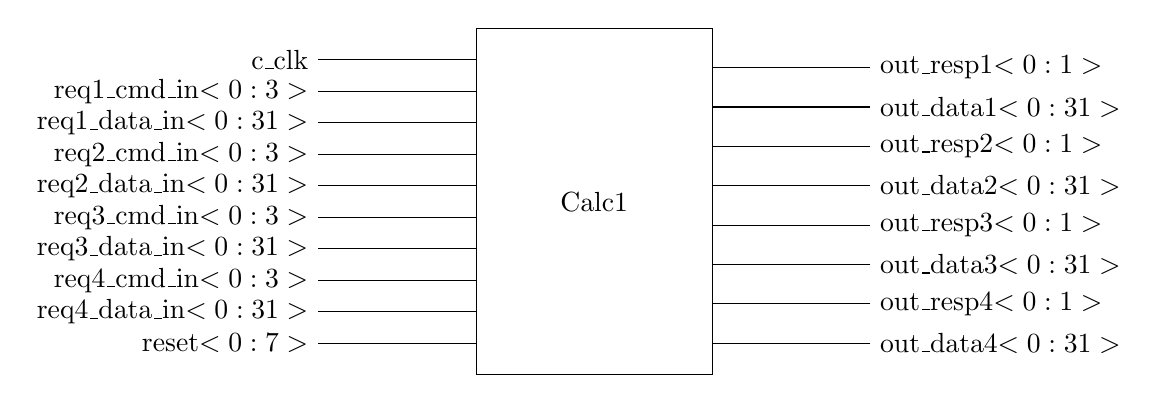
\begin{tikzpicture}
        \node (rectangle) [draw, rectangle, minimum width = 3 cm, minimum
        height = 4.4 cm] (Y) at (4,0) {Calc1} ;
        \draw [-] ($(Y.west) + (0,1.8)$) -- ++ (-2, 0) node [pos = 1, left]
        {c\_clk};
        \draw [-] ($(Y.west) + (0,1.4)$) -- ++ (-2, 0) node [pos = 1, left]
        {req1\_cmd\_in$<0:3>$};
        \draw [-] ($(Y.west) + (0,1.0)$) -- ++ (-2, 0) node [pos = 1, left]
        {req1\_data\_in$<0:31>$};
        \draw [-] ($(Y.west) + (0,0.6)$) -- ++ (-2, 0) node [pos = 1, left]
        {req2\_cmd\_in$<0:3>$};
        \draw [-] ($(Y.west) + (0,0.2)$) -- ++ (-2, 0) node [pos = 1, left]
        {req2\_data\_in$<0:31>$};
        \draw [-] ($(Y.west) + (0,-0.2)$) -- ++ (-2, 0) node [pos = 1, left]
        {req3\_cmd\_in$<0:3>$};
        \draw [-] ($(Y.west) + (0,-0.6)$) -- ++ (-2, 0) node [pos = 1, left]
        {req3\_data\_in$<0:31>$};
        \draw [-] ($(Y.west) + (0,-1.0)$) -- ++ (-2, 0) node [pos = 1, left]
        {req4\_cmd\_in$<0:3>$};
        \draw [-] ($(Y.west) + (0,-1.4)$) -- ++ (-2, 0) node [pos = 1, left]
        {req4\_data\_in$<0:31>$};
        \draw [-] ($(Y.west) + (0,-1.8)$) -- ++ (-2, 0) node [pos = 1, left]
        {reset$<0:7>$};
        \draw [-] ($(Y.east) + (2,1.7)$) -- ++ (-2, 0) node [pos = 0, right]
        {out\_resp1$<0:1>$};
        \draw [-] ($(Y.east) + (2,1.2)$) -- ++ (-2, 0) node [pos = 0, right]
        {out\_data1$<0:31>$};
        \draw [-] ($(Y.east) + (2,0.7)$) -- ++ (-2, 0) node [pos = 0, right]
        {out\_resp2$<0:1>$};
        \draw [-] ($(Y.east) + (2,0.2)$) -- ++ (-2, 0) node [pos = 0, right]
        {out\_data2$<0:31>$};
        \draw [-] ($(Y.east) + (2,-0.3)$) -- ++ (-2, 0) node [pos = 0, right]
        {out\_resp3$<0:1>$};
        \draw [-] ($(Y.east) + (2,-0.8)$) -- ++ (-2, 0) node [pos = 0, right]
        {out\_data3$<0:31>$};
        \draw [-] ($(Y.east) + (2,-1.3)$) -- ++ (-2, 0) node [pos = 0, right]
        {out\_resp4$<0:1>$};
        \draw [-] ($(Y.east) + (2,-1.8)$) -- ++ (-2, 0) node [pos = 0, right]
        {out\_data4$<0:31>$};
    \end{tikzpicture}
    \caption{Calc1 inputs and outputs diagram}
    \label{figure:1}
\end{figure}
\noindent Calc1 command decode values are shown in Table~\ref{table:1}.
\begin{table}[H]
    \centering
    \begin{tabular}{ll}
        \toprule
        Command & Decode value \\
        \cmidrule(r){1-1}\cmidrule(lr){2-2}
        No operation & "0000"b\\
        Add & "0001"b\\
        Subtract & "0010"b\\
        Shift left & "0101"b\\
        Shift right& "0110"b\\
        Invalid & All others\\
        \bottomrule
    \end{tabular}
    \caption{Calc1 command decode values}
    \label{table:1}
\end{table}
Bits shifted out of operations on this design are dropped and zeros are shifted
in. Only the least significant bits of the second operand are taken into
account for the shifting operations. Calc1 response values are shown in
Table~\ref{table:2}.
\begin{table}[H]
    \centering
    \begin{tabular}{lp{12cm}l}
        \toprule
        Response decode & Response meaning\\
        \cmidrule(r){1-1}\cmidrule(lr){2-2}
        "00"b & No response on this cycle. \\
        "01"b & Successful response. Response data are on the output bus.\\
        "10"b & Overflow, underflow or invalid command. Overflow/underflow only
        valid for the add or subtract commands. No data on output data bus.\\ 
        "11"b & Unused response value. \\
        \bottomrule
    \end{tabular}
    \caption{Calc1 command decode values}
    \label{table:2}
\end{table}
Each port is independent of other. If all ports send commands concurrently, the
response may not be concurrent. Also there is a limitation of functional units
inside this design so similar commands will be serialized and processed one at
a time. This scheme calculates commands on FCFS basis. Calc1 will not order
commands arriving on the same clock on a particular basis. \\
During verification reset line should be set to "1111111"b for 7 consecutive 
clock cycles to reset the design. Calc1 treats operands as unsigned data.
The way inputs work is that we should put the request command and the first
operand in one cycle and then we put the second operand on the next cycle. The
design will answer on later clocks at its leisure. Also we have one ALU for
adds and subtracts, and a second ALU for shifting commands. This implies that
we can only have one operation on each ALU output at the same time. Each port 
should wait for the answer before sending another command.

\subsection{Verification scenarios}
Here we have some verification scenarios which are based on the examples of the
book. \\
\begin{table}[H]
    \centering
    \begin{tabular}{lp{12cm}l}
        \toprule
        Test refrence number& Test description\\
        \cmidrule(r){1-1}\cmidrule(lr){2-2}
        1.1 & Check the basic command response of the four ports. \\
        1.2 & Check the basic operation of each command on each port.\\
        1.3 & Check the overflow and underflow cases for add and subtracts \\
        2.1.1 & For each port, check that each command can have any command
        follow it without leaving the design dirty. \\
        2.1.2 & Across all ports check that after a same command like all adds
        we can have another command without leaving the design dirty. \\
        2.2 & Check that there is fairness across all ports such that no port
        has higher priority than others. \\
        2.3 & Check that the high-order 27 bits are ignored in the second
        operand for the shift commands. \\
        2.4.1 & Add two numbers that overflows by 1 \\
        2.4.2 & Add two numbers whose sum is "FFFFFFFF"X \\
        2.4.3 & Subtract two equal numbers. \\
        2.4.4 & Subtract a number that underflows by 1. \\
        2.4.5 & Shift 0 places. \\
        2.4.6 & Shift 31 places. \\
        2.5 & Check that the design ignores data inputs unless the data are
        supposed to be valid, in other words check that the design latches the
        data only when appropriate.\\
        3.1 & Check that the design handles illegal commands\\
        3.2 & Check all outputs all of the time so that Calc1 does not output
        errorneos output values.\\
        3.3 & Check that the reset function correctly resets the design.\\
        \bottomrule
    \end{tabular}
    \caption{Calc1 function test}
    \label{table:3}
\end{table}

\section{Calc2 Design Description}

\subsection{Overview of the system}
Calc2 behaves similarly to the Calc1 design. But unlike Calc1 we will not wait
for the completion of the last command. So in each port we can send up to four
concurrent commands. Out of order execution is possible because we have two
functional units. However the specifications dictate that the results return in
order of the commands that has been issued. To correlate the responses to their
issued command there is a 2 bit tag to the input and output protocol. This tag
should be a unique identifier therefore each port requester should keep track
of the tags and should not allow duplicate tags. Figure~\ref{figure:2} is self
explanatory and shows the inputs and outputs. There are four sets of inputs and
outputs which correlate to the command, data, and the tag inputs and outputs.
Also we should not let the similarities between Calc1
and Calc2 deceive us as it should be studied like an independent design.
\begin{figure}[H]
    \centering
    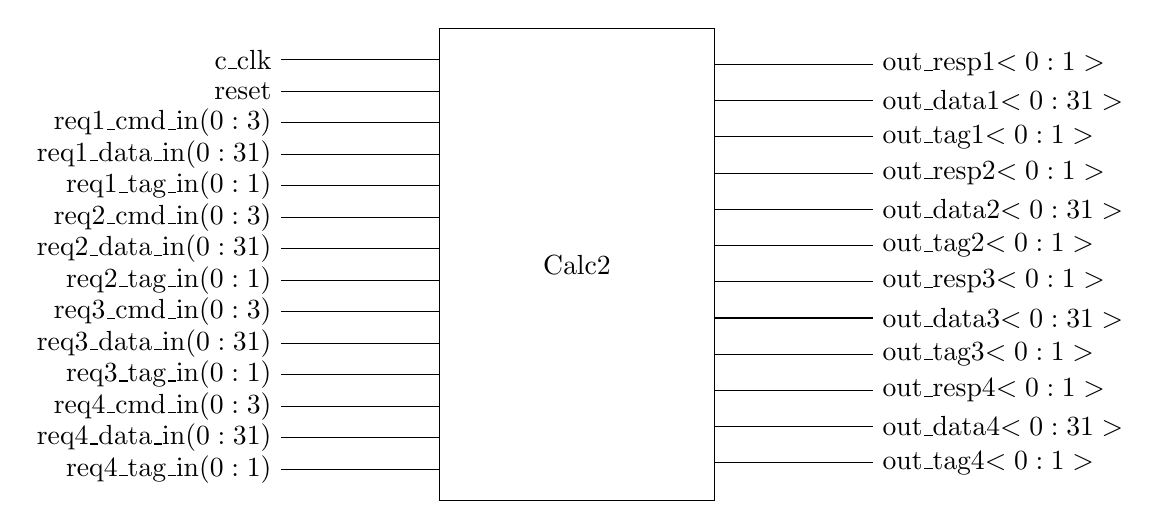
\begin{tikzpicture}
        \node (rectangle) [draw, rectangle, minimum width = 3.5 cm, minimum
        height = 6 cm] (Y) at (4,0) {Calc2} ;
        \draw [-] ($(Y.west) + (0,2.6)$) -- ++ (-2, 0) node [pos = 1, left]
        {c\_clk};
        \draw [-] ($(Y.west) + (0,2.2)$) -- ++ (-2, 0) node [pos = 1, left]
        {reset};
        \draw [-] ($(Y.west) + (0,1.8)$) -- ++ (-2, 0) node [pos = 1, left]
        {req1\_cmd\_in$(0:3)$};
        \draw [-] ($(Y.west) + (0,1.4)$) -- ++ (-2, 0) node [pos = 1, left]
        {req1\_data\_in$(0:31)$};
        \draw [-] ($(Y.west) + (0,1.0)$) -- ++ (-2, 0) node [pos = 1, left]
        {req1\_tag\_in$(0:1)$};
        \draw [-] ($(Y.west) + (0,0.6)$) -- ++ (-2, 0) node [pos = 1, left]
        {req2\_cmd\_in$(0:3)$};
        \draw [-] ($(Y.west) + (0,0.2)$) -- ++ (-2, 0) node [pos = 1, left]
        {req2\_data\_in$(0:31)$};
        \draw [-] ($(Y.west) + (0,-0.2)$) -- ++ (-2, 0) node [pos = 1, left]
        {req2\_tag\_in$(0:1)$};
        \draw [-] ($(Y.west) + (0,-0.6)$) -- ++ (-2, 0) node [pos = 1, left]
        {req3\_cmd\_in$(0:3)$};
        \draw [-] ($(Y.west) + (0,-1.0)$) -- ++ (-2, 0) node [pos = 1, left]
        {req3\_data\_in$(0:31)$};
        \draw [-] ($(Y.west) + (0,-1.4)$) -- ++ (-2, 0) node [pos = 1, left]
        {req3\_tag\_in$(0:1)$};
        \draw [-] ($(Y.west) + (0,-1.8)$) -- ++ (-2, 0) node [pos = 1, left]
        {req4\_cmd\_in$(0:3)$};
        \draw [-] ($(Y.west) + (0,-2.2)$) -- ++ (-2, 0) node [pos = 1, left]
        {req4\_data\_in$(0:31)$};
        \draw [-] ($(Y.west) + (0,-2.6)$) -- ++ (-2, 0) node [pos = 1, left]
        {req4\_tag\_in$(0:1)$};
        \draw [-] ($(Y.east) + (2,2.54)$) -- ++ (-2, 0) node [pos = 0, right]
        {out\_resp1$<0:1>$};
        \draw [-] ($(Y.east) + (2,2.08)$) -- ++ (-2, 0) node [pos = 0, right]
        {out\_data1$<0:31>$};
        \draw [-] ($(Y.east) + (2,1.62)$) -- ++ (-2, 0) node [pos = 0, right]
        {out\_tag1$<0:1>$};
        \draw [-] ($(Y.east) + (2,1.16)$) -- ++ (-2, 0) node [pos = 0, right]
        {out\_resp2$<0:1>$};
        \draw [-] ($(Y.east) + (2,0.7)$) -- ++ (-2, 0) node [pos = 0, right]
        {out\_data2$<0:31>$};
        \draw [-] ($(Y.east) + (2,0.24)$) -- ++ (-2, 0) node [pos = 0, right]
        {out\_tag2$<0:1>$};
        \draw [-] ($(Y.east) + (2,-0.22)$) -- ++ (-2, 0) node [pos = 0, right]
        {out\_resp3$<0:1>$};
        \draw [-] ($(Y.east) + (2,-0.68)$) -- ++ (-2, 0) node [pos = 0, right]
        {out\_data3$<0:31>$};
        \draw [-] ($(Y.east) + (2,-1.14)$) -- ++ (-2, 0) node [pos = 0, right]
        {out\_tag3$<0:1>$};
        \draw [-] ($(Y.east) + (2,-1.60)$) -- ++ (-2, 0) node [pos = 0, right]
        {out\_resp4$<0:1>$};
        \draw [-] ($(Y.east) + (2,-2.06)$) -- ++ (-2, 0) node [pos = 0, right]
        {out\_data4$<0:31>$};
        \draw [-] ($(Y.east) + (2,-2.52)$) -- ++ (-2, 0) node [pos = 0, right]
        {out\_tag4$<0:1>$};
    \end{tikzpicture}
    \caption{Calc2 inputs and outputs diagram}
    \label{figure:2}
\end{figure}
Reset also should be held up for seven consecutive cycles as it was in Calc1.
The operation of sending data and commands should be done in two clock cycles.
In the first clock we put command, tag in, and first operand. 
Then in the second cycle we send the second operand. 

\subsection{Verification scenarios}
Here we have some verification scenarios which are based on the examples of the
book. All the scenarios described in the Calc1 also apply to the Calc2.
\begin{table}[H]
    \centering
    \begin{tabular}{lp{12cm}l}
        \toprule
        Test refrence number& Test description\\
        \cmidrule(r){1-1}\cmidrule(lr){2-2}
        4.1 & Send multiple commands with variable timing between commands
        for the same port. \\
        4.2 & Send commands using variable tags for each commands. \\
        4.3 & Send multiple invalid commands. \\
        5.1 & Send only a mix of add and subtract commands to fill the add
        queue. \\
        5.2 & Send only a mix of shift commands to fill the shift queue. \\
        5.3 & Verify mixes of overflow, underflow and good response cases
        across back to back port commands. \\ 
        5.4 & Verify all lenghts of shift cases across back to back port 
        commands. \\ 
        5.5 & Verify the design under verfication does not allow output
        collisions from both pipelines sending results to the same port
        simultaneously.\\
        \bottomrule
    \end{tabular}
    \caption{Calc1 function test}
    \label{table:4}
\end{table}

\bibliographystyle{abbrv}
% \bibliography{references}  % need to put bibtex references in references.bib 
\end{document}
